\documentclass{article}
\usepackage{graphicx}
\usepackage{siunitx}
\usepackage{hyperref}
\graphicspath{ {images/} }
\title{Maximum Speed Flat Turn}
\author{Grant Curell}
\begin{document}
\maketitle{}
\section{Problem}
Say you’re sitting in the passenger seat of the car, approaching a turn with a 200.0-meter radius (with a level, non-banked road surface). You know that the coefficient of static friction is 0.8 on this road (you use the coefficient of static friction because the tires aren’t slipping on the road’s surface) and that the car has a mass of about 1,000 kilograms. What’s the maximum speed the driver can go and still keep you safe?
\\\\
Holzner, Steven. Physics I For Dummies (For Dummies (Math \& Science)) (p. 123). Wiley. Kindle Edition.
\\\\
\section{Proof of \[a_c=\frac{a^2}{r} \]}
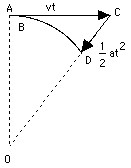
\includegraphics[width=\columnwidth]{triangle}
\[ R^2+(vt)^2=(R+x)^2 \]
Holy shit I actually have to remember how to FOIL. Do you know how many years it has been since I used FOIL?
\[ R^2+(vt)^2=R^2+2Rx+x^2 \]
\[ (vt)^2=2Rx+x^2 \]
\[ \lim_{t\to0} x(2R+x)=v^2t^2 \]
I don't full understand the above. I got the original proof from \url{http://www.phy6.org/stargaze/Mcircul.htm}, \url{http://www.phy6.org/stargaze/Scircul.htm} for english. Why does that not get you zero overall? Admittedly, it has been 7 or 8 years since I last did a limit. Am going to follow up.
\[ v^2t^2=2xR \]
\[ \frac{v^2t^2}{2R}=x \]
That somehow gets simplified to:
\[ a=\frac{v^2}{R} \]
\section{Problem}
\[ r=200m \]
\[ \mu_s=.8 \]
\[ m=1000kg \]
The idea is we figure out how much force the tires can apply via friction and use that to derive acceleration which I can tie to a max velocity.
\[ F_{friction}=ma \]
\[F_{friction}=m*g*\mu_s \]
\[ F_{friction}=1000*9.8*.8 \]
\[ F_{friction}=7840N \]
7840N is the maximum force the tires can apply to the road.
\[ 7840 = m*a_c \]
\[ 7840 = 1000*\frac{v^2}{200} \]
\[ v = 40 m/s \]
\end{document}
